\section{Auswertung}
\label{sec:Auswertung}
Die für den Versuch relevanten Bauteile haben die Werte
\begin{eqnarray}
  L 	&= (\num{16.78 +- 0.09}) mH	\\
  C 	&= (\num{2.066 +- 0.006}) nF	\\
R_1 	&= (\num{67.2 +- 0.2}) \Omega	\\
R_2 	&= (\num{682 +- 1}) \Omega
  \label{eqn:Bau}
\end{eqnarray}

\subsection{Zeitabhänigkeit der Amplitude und Dämpfungswiederstand einer Gedämpften Schwingung}
Die durch das Oszilliskop gemessene Spannungspeaks werden mittels einer CWD-Funktion ermittelt und mit deren dazugehörige Zeit in Tabelle \ref{tab:U_C} aufgetragen.
\begin{table}
  \centering
  \begin{tabular}{c c}
    \toprule
    	$U_\text{C}$ / V & $t$ / $10^{-3}$ \\
    \midrule
	52	& 0.18	\\
	48.8	& 0.54	\\
	45.6	& 0.93 	\\
	41.6	& 1.30	\\
	38.4	& 1.69	\\
	36.6	& 2.09 	\\
	34.2	& 2.46	\\
	33.3 	& 2.82	\\
	32	& 3.20 	\\
	31.4	& 3.59	\\
	29.6	& 3.96	\\
	28.8	& 4.32 	\\
    \bottomrule
  \end{tabular}
  \caption{Spannung am Kondensator zur Bestimmung des Abklingverhalten und Dämpfungswiederstand.}
  \label{tab:U_C}
\end{table}
Anhand der Daten lässt sich durch eine Fit-Funktion die Koeffizienten der Einhüllenden berechnen, welche in Gleichung ?? beschrieben sind. 
\begin{eqnarray}
  A_0 = ( \num{30.6 +- 0.9} ) \text{V} \\
  f = ( \num{680 +- 60} ) \text{Hz}
  \label{eqn:Koef}
\end{eqnarray}
Die Einhüllende und die Messdaten sind in Abbildung \ref{fig:Osz} dargestellt.
\begin{figure}
  \centering
  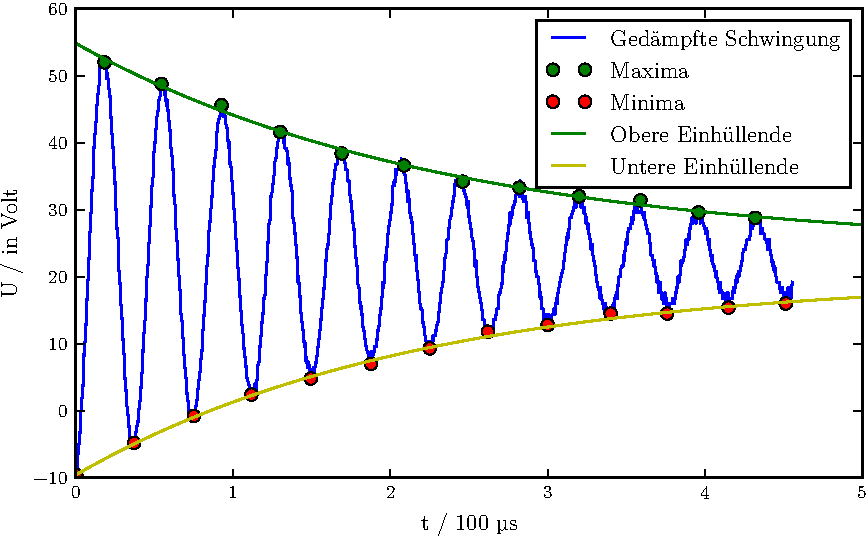
\includegraphics[height=5cm]{plot.pdf}
  \caption{Messdaten mit Einhüllender}
  \label{fig:Osz}
\end{figure}
Nach Formel ?? lässt sich der effektive Dämpfungswiederstand sowie die Abklingdauer berechnen.
\begin{eqnarray}
  R_\text{eff} = ( \num{143.38 +- 12.7}) \, \Omega \\
  T_\text{ex} = ( \num{230 +- 10}) \cdot 10^{-6} \, \text{s}
  \label{eqn:Reff}
\end{eqnarray}
Der Erwatungswert wiegt vom Errechneten wert um 75 $\Omega$ ab. Dies lässt sich einerseits dadurch erklären, dass der Innenwiederstand von 50 $\Omega$ nicht berücksichtigt wurde. Andererseits kann es bei der gewählten Frequenz zu Impedanzen der verschiedenen Bauteile gekommen sein. Für die weiteren Aufgaben wird der Widerstand des Generators berücksichtigt.
\subsection{Dämpfungswiederstand des Aperiodischen Grenzfalls}
Der im Experiment bestimmte Widerstand, bei dem der Aperiodische Grenzfall eintritt, beträgt
\begin{equation}
  R_\text{Praxis} = 1.25 \, \Omega \ .
  \label{eqn:Rprax}
\end{equation}
Der Theoretische Widerstand wird mittels Formel ?? ausgerechnet und beträgt 
\begin{equation}
  T_\text{Theorie} = (\num{2.75 +- 0.23}) , \Omega \ .
  \label{eqn:Rthe}
\end{equation}
Zwischen dem theoretischen und praktisch ermittelten ist eine Differenz von 1.5 $\Omega$. Mögliche Ursachen für den Fehler sind, die vernachlässigte Impedanz des Aufbaus, als auch die Schwierigkeit den Punkt des Aperiodischen Grenzfalls zu treffen, da keine wesentliche Änderung erkennen zu sind. 
\subsection{Frequenzabhängigkeit der Kondensatorspannung eines  Serienresonanzkreis}
In Tabelle \ref{tab:U_c} sind die Spannung am Kondensator und die entsprechenden Frequenzen hinterlegt.
\begin{table}
  \centering
  \begin{tabular}{c c}
	\toprule
	f / Hz & U / V \\
	\midrule
	9	& 5.6	\\
	12	& 6.4	\\
	16	& 6.8	\\
	23	& 7.2	\\
	35	& 7.2	\\
	61	& 7.6	\\
	162	& 7.6	\\
	307	& 7.6	\\
	500	& 7.6	\\
	905	& 7.6	\\
	1604	& 7.8	\\
	2509	& 7.8	\\
	4025	& 7.8	\\
	5615	& 8.0	\\
	8970	& 9.0	\\
 	12030	& 10.0	\\
 	15400	& 11.2	\\
 	17610	& 13.0	\\
 	20000	& 15.6	\\
 	22520	& 20.4	\\
 	24000	& 24.8	\\
	24490	& 26.0	\\
	25180	& 27.6	\\
	25570	& 28.0	\\
	26300	& 28.4	\\
	27060	& 27.2	\\
 	27610	& 26.0	\\
 	28100	& 24.2	\\
 	29970	& 18.0	\\
 	32540	& 12.4	\\
	35660	& 8.6	\\
	40030 	& 5.4	\\
	42580 	& 4.4	\\
	45000	& 3.7	\\
	50180	& 2.7	\\
	52430 	& 2.4	\\
	55010	& 2.2	\\
	\bottomrule
 	\end{tabular}
  \caption{Frequanzabhängigkeit der Kondensatorspannung}
  \label{tab:U_c}
\end{table}
Anhand derer und der Abbildung \ref{fig:logUc} lässt sich der maximalwert der Güte ablesen. Er beträgt
\begin{equation}
  q_\text{exp} = 28.4 \ .
  \label{eqn:qexp}
\end{equation}
Anhand Formel ?? lässt sich der theoretische Güte ausrechnen. Sie beträgt 
\begin{equation}
  q_\text{theo} = (\num{4.18 +- 0.01})
  \label{eqn:qtheo}
\end{equation} 
und ist somit 579 \% größer als der Praktisch ermittelte Wert. Mittels eines linearen Plot (siehe Abbildung \ref{fig:fUc}) soll die breite der Resonanzkurve bestimmt werden. Durch Ablesen wird die Breite der Resonanzkurve bestimmt welche 
\begin{equation}
  v_+ - v_- = 6.72 \, \text{kHz} 
\end{equation}
entspricht. Die theoretische breite berechnet sich nach Formel ?? berechnet. Sie beträgt 
\begin{equation}
v_+ - v_- = (\num{6.47 +- 0.04}) \, \text{kHz} \ .
\end{equation}
Der experimentell bestimmte weicht vom theoretischen Wert um 3.9 \% ab.
\begin{figure}
  \centering
  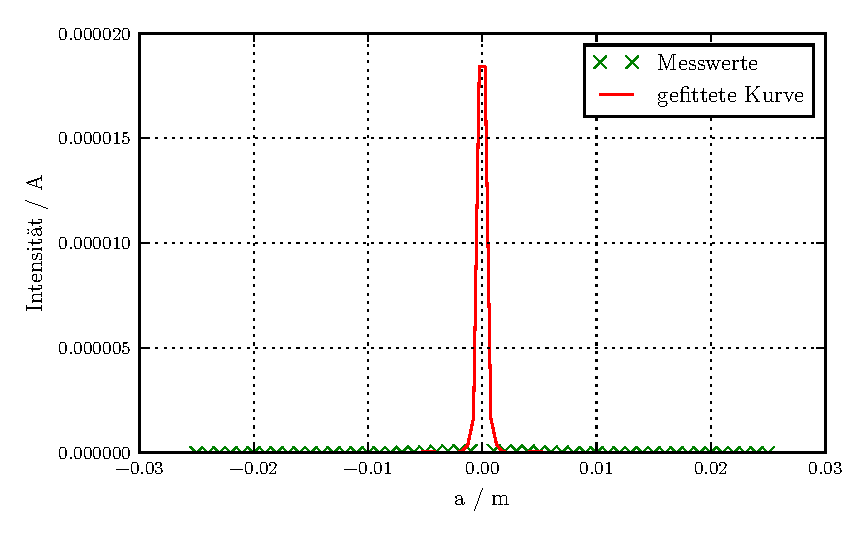
\includegraphics[height=5cm]{plot1.pdf}
  \caption{Halblogaritmisch aufgetragene Kondensatorspannung gegen die Frequenz}
  \label{fig:logUc}
\end{figure}

\begin{figure}
  \centering
  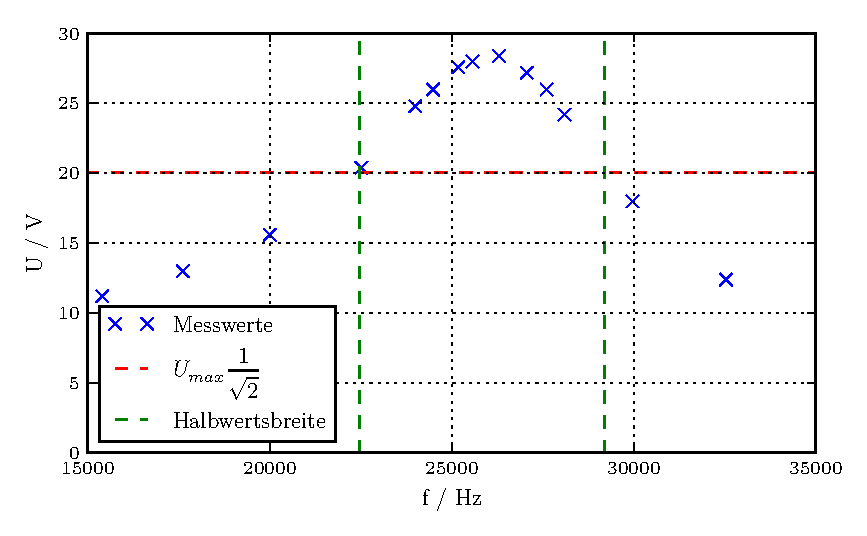
\includegraphics[height=5cm]{plot2.pdf}
  \caption{Frequenzabhängige Kondensatorspannung}
  \label{fig:fUc}
\end{figure}

